\documentclass{article}
\usepackage{tikz}
\usepackage{pgfplots}
\usepgfplotslibrary{statistics}
\usepackage{xcolor}
\usepackage{geometry}
\geometry{margin=1in}

% Define grayscale colors
\definecolor{regionA}{gray}{0.85}
\definecolor{regionB}{gray}{0.7}
\definecolor{regionC}{gray}{0.55}
\definecolor{regionD}{gray}{0.4}
\definecolor{regionE}{gray}{0.25}
\definecolor{regionF}{gray}{0.1}

% New legend box style
\newcommand{\legendbox}[2]{%
	\begin{tikzpicture}[baseline={(0,-0.5ex)}]
		\filldraw[#1] (0,0) rectangle (1em,1em);
		\node[anchor=west] at (1.2em,0.5em) {#2};
	\end{tikzpicture}
}

\begin{document}
	
	\begin{figure}
		\centering
		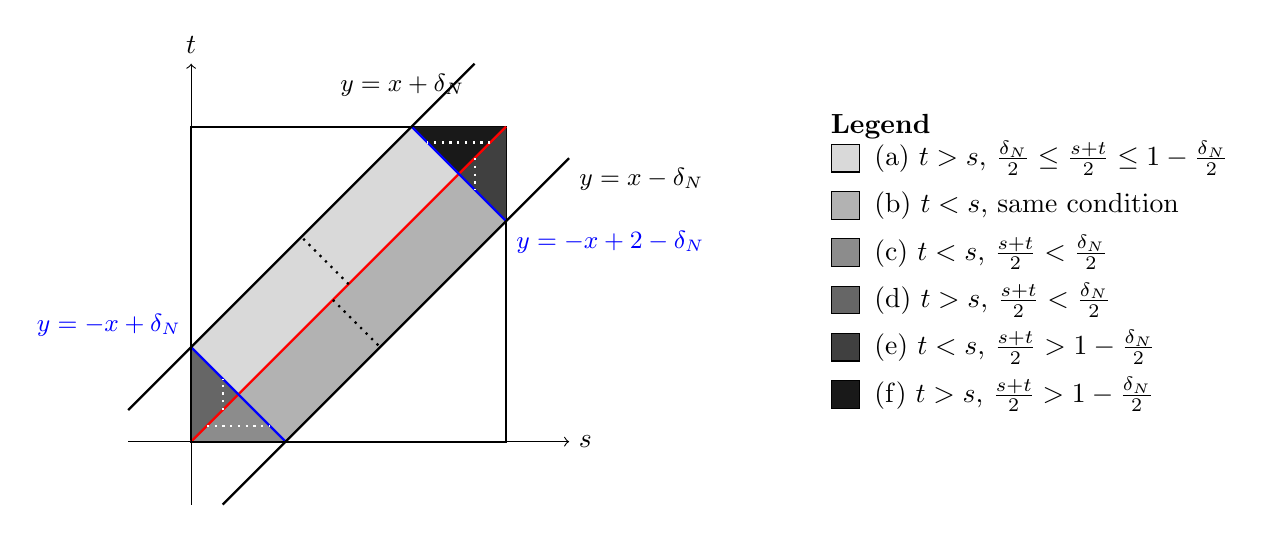
\begin{tikzpicture}[scale=4]
			\def\dd{0.3}
			
			% Square and regions
			\draw[thick] (0,0) rectangle (1,1);
			
			\fill[regionC] (0,0) -- (\dd,0) -- (\dd/2,\dd/2) -- cycle;
			\fill[regionE] (1,1-\dd) -- (1,1) -- (1-\dd/2,1-\dd/2) -- cycle;
			\fill[regionD] (0,0) -- (0,\dd) -- (\dd/2,\dd/2) -- cycle;
			\fill[regionF] (1-\dd,1) -- (1,1) -- (1-\dd/2,1-\dd/2) -- cycle;
			\fill[regionB] (\dd,0) -- (\dd/2,\dd/2) -- (1-\dd/2,1-\dd/2) -- (1,1-\dd) -- cycle;
			\fill[regionA] (0,\dd) -- (\dd/2,\dd/2) -- (1-\dd/2,1-\dd/2) -- (1-\dd,1) -- cycle;
			
			% Reference lines
			\draw[red, thick] (0,0) -- (1,1);
			\draw[blue, thick] (\dd,0) -- (0,\dd) node[above left] {\small $y=-x+\delta_N$};
			\draw[blue, thick] (1-\dd,1) -- (1,1-\dd) node[below right] {\small $y=-x+2-\delta_N$};
			\draw[black, thick] (-0.2+\dd,-0.2) -- (1.2,1.2-\dd) node[below right] {\small $y=x-\delta_N$};
			\draw[black, thick] (-0.2, -0.2+\dd) -- (1.2-\dd,1.2) node[below left] {\small $y=x+\delta_N$};
			
			\draw[dotted, thick, white] (\dd/3, \dd/3) -- (\dd/3,\dd-\dd/3);
			\draw[dotted, thick, white] (\dd/6, \dd/6) -- (\dd-\dd/6,\dd/6);
			\draw[dotted, thick, white] (1-\dd/3, 1-\dd/3) -- (1-\dd/3,1-\dd+\dd/3);
			\draw[dotted, thick, white] (1-\dd/6, 1-\dd/6) -- (1-\dd+\dd/6,1-\dd/6);
			\draw[dotted, thick] (1/2, 1/2) -- (1/2-\dd/2,1/2+\dd/2);
			\draw[dotted, thick] (1/2-\dd/6, 1/2-\dd/6) -- (1/2-\dd/6+\dd/2,1/2-\dd/6-\dd/2);
			
			% Axes
			\draw[->] (-0.2,0) -- (1.2,0) node[right] {$s$};
			\draw[->] (0,-0.2) -- (0,1.2) node[above] {$t$};
			
			% Legend box to the far right
			\begin{scope}[shift={(2,-0.1)}]
				\node[anchor=west] at (0,1.1) {\textbf{Legend}};
				\node[anchor=west] at (0,1.0) {\legendbox{fill=regionA}{(a) $t > s$, $\frac{\delta_N}{2} \leq \frac{s+t}{2} \leq 1 - \frac{\delta_N}{2}$}};
				\node[anchor=west] at (0,0.85) {\legendbox{fill=regionB}{(b) $t < s$, same condition}};
				\node[anchor=west] at (0,0.7) {\legendbox{fill=regionC}{(c) $t < s$, $\frac{s+t}{2} < \frac{\delta_N}{2}$}};
				\node[anchor=west] at (0,0.55) {\legendbox{fill=regionD}{(d) $t > s$, $\frac{s+t}{2} < \frac{\delta_N}{2}$}};
				\node[anchor=west] at (0,0.4) {\legendbox{fill=regionE}{(e) $t < s$, $\frac{s+t}{2} > 1 - \frac{\delta_N}{2}$}};
				\node[anchor=west] at (0,0.25) {\legendbox{fill=regionF}{(f) $t > s$, $\frac{s+t}{2} > 1 - \frac{\delta_N}{2}$}};
			\end{scope}
		\end{tikzpicture}
		\caption{%
			Definition of domains in $\mathcal{D}$ for the estimator $\widehat{\Gamma}_{N, 0}^*(s,t)$. Each region (a)–(f) is shaded in grayscale and defined in the legend to the right.
		}
		\label{fig:def_cov_diagBand}
	\end{figure}
	
\end{document}
